% ----------------------------- CONCETTI AVANZATI ------------------------------------

\chapter{Concetti Avanzati}

% Argomenti di questo capitolo da trattare:

%TODO: Signal Handling? (magari in un capitolo sul multithreading)

%TODO: Writing C++ code efficiently in Competitive Programming? (magari in un capitolo apposito)

%TODO: Dependency Injection

%TODO: std::bad_alloc (Insomma, non necessaria per sto capitolo credo)

%TODO: magari aggiungere nel capitolo "basi del linguaggio": struct destructors che servono se allochi della memoria nelle struct, non se le usi, ma se allochi.

%TODO: xvalue? (oppure lo aggiungo quando parlo di lvalue e rvalue)

%TODO: performance optimization, performance, optimization techniques?
%TODO: un esempio è usare ++i al posto di i++
%TODO: esempi: Premature Pessimization to avoid Premature Optimization.

%TODO: template metaprogramming? (nel capitolo dei Design Patterns)

% -------------------------- SECTION: INTRODUZIONE -----------------------------------

\section{Introduzione}

\textsf{\small In questo capitolo "finale" tratterò argomenti un po' più complessi o che almeno non mi verrebbe da mettere negli altri due capitoli precedenti.} \\

\textsf{\small Verranno trattati argomenti come gli smart pointers e quindi unique pointers, share pointers, weak pointers, le friend function e altri importanti concetti avanzati.} \\

% -------------------------- SECTION: FRIEND KEYWORD ---------------------------------

\newpage

\section{Friend Keyword}

\subsection{Friend Class}

\textsf{\small \textbf{Definizione: } La keyword \textbf{friend} è usata per accedere ai membri privati e protetti di una classe nella quale è dichiarata \textbf{friend}.} \\

\begin{lstlisting}
	#include <iostream>
	
	class A {
		public:
			A() { a = 0 };
			friend class B; // Classe amica.
			
		private:
			int a;
	};

	class B {
		public:
			void showA(A& x)
			{
				// Visto che B è un'amica di A, può accedere ai membri privati di A.
				std::cout << "A::a : " << x.a; 
			}
	};

	int main()
	{
		A a;
		B b;
		b.showA(); //Output: A::a : 0
		return 0;
	}
\end{lstlisting}

\subsection{Friend Function}

\textsf{\small \textbf{Definizione: } Come per le \textbf{classi friend}, una \textbf{funzione friend} ha accesso speciale ai membri privati e protetti.} \\

\textsf{\small Una \textbf{friend function} può essere: } \\

\begin{itemize}
	\item \textsf{\small Un membro di un'altra classe.}
	\item \textsf{\small Una funzione globale.}
\end{itemize}

\textsf{\small Alcuni importanti punti riguardo alle \textbf{friend} functions e classes: } \\

\begin{itemize}
	\item \textsf{\small Dovrebbero essere usate solo in maniera limitata. Troppe funzioni o classi \textbf{friend} diminuiscono l'encapsulazione.}
	\item \textsf{\small L'amicizia non è reciproca. Se la classe A è amica della classe B, allora B non è automaticamente amica di A.}
	\item \textsf{\small L'amicizia non è ereditata.}
	%\item \textsf{\small }
\end{itemize}

\begin{lstlisting}
	#include <iostream>
	
	class A {
		public:
			friend void printWidth( A a);
			void setWidth(double w);
			
		private:
			double width;
	};

	// Definizione della funzione membro di A.
	void A::setWidth(double w)
	{
		width = w;
	}

	// printWidth non è una funzione membro di nessuna classe.
	void printWidth( A a )
	{
		// Visto che la funzione printWidth è amica di A, può accedere direttamente a qualsiasi membro di A.
		std::cout << "Width di A: " << a.width << std::endl;
	}

	int main()
	{
		A a;
		
		a.setWidth(11.1);
		
		// Uso la funzione amica per stampare la width di a.
		printWidth( a ) ; //Output: Width di A: 11.1
		return 0;
	}
\end{lstlisting}

% -------------------------- SECTION: SMART POINTERS ---------------------------------

\newpage

\section{Smart Pointers}

\textsf{\small \textbf{Definizione: } Gli \textbf{smart pointers} (puntatori intelligenti) sono dei puntatori che, in più rispetto ai normali puntatori, sono in grado di deallocare la memoria automaticamente, senza che il programmatore debba occuparsene ed evitando \emph{memory leak}.} \\

\subsection{Differenze con i puntatori normali}

\textsf{\small I \textbf{puntatori} servono per poter accedere a delle risorse che sono esterne al programma (alla memoria heap). Grazie ai puntatori saremo in grado di modificare direttamente la risorsa esterna, al posto di doverne fare una copia.} \\

\textsf{\small Il problema di questi puntatori è che se non deallocati correttamente potrebbero portare ad uno spreco della memoria heap, il che è un \emph{memory leak}.} \\

\begin{lstlisting}
	#include <iostream>
	
	class Rectangle {
		private:
			int width;
			int height;
	};

	void fun()
	{
		Rectangle* p = new Rectangle();
	}

	int main()
	{
		while(1)
		{
			fun();
		}
		//Output: Il problema è che quando la funzione fun termina, il puntatore p verrà distrutto come fosse una variabile locale, ma la memoria allocata non verrà deallocata, perché ci siamo scordati di usare \emph{delete p}; alla fine della funzione.
		
		// Ciò è un problema perché verrà sempre allocata altra memoria e mai deallocata, occupando spazio, sprecando memoria, il che è un \emph{memory leak}.
		
		// L'intera memoria heap potrebbe diventare inutile per questo motivo. 
		return 0;
	}
\end{lstlisting}

\textsf{\small Il problema è che quando la funzione fun termina, il puntatore p verrà distrutto come fosse una variabile locale, ma la memoria allocata non verrà deallocata, perché ci siamo scordati di usare \emph{delete p}; alla fine della funzione.} \\

\textsf{\small Ciò è un problema perché verrà sempre allocata altra memoria e mai deallocata, occupando spazio, sprecando memoria, il che è un \emph{memory leak}.} \\

\textsf{\small L'intera memoria heap potrebbe diventare inutile per questo motivo. } \break

\textsf{\small Uno \textbf{smart pointer} è un \emph{wrapper} (un wrapper è un'entità che ne encapsula un'altra; è del codice che letteralmente avvolge, incarta, impacchetta, confeziona dell'altro codice) su un puntatore con un'operatore \textbf{*} e \textbf{->} overloaded.} \\

\textsf{\small La memoria allocata dinamicamente verrebbe così automaticamente liberata.} \\

\begin{lstlisting}
	// Una generica classe Smart Pointer
	#include <iostream>
	
	template <class T>
	class SmartPointer {
		T *ptr;
		public:
			SmartPointer(T *ptr = NULL)
			{
				p = ptr;
			}
		
			~SmartPointer()
			{
				delete ptr;
			}
		
			T & operator * ()
			{
				return *ptr;
			}
		
			T * operator ->()
			{
				return ptr;
			}
	};

	int main()
	{
		SmartPointer<int> p(new int());
		*p = 22;
		std::cout << "Valore di *p: " << *p << std::endl; //Output: Valore di *p: 22
		return 0;
	}
\end{lstlisting}

%TODO: dynamic_pointer_cast
%TODO: const_pointer_cast

\subsection{unique pointers}

\textsf{\small \textbf{Definizione: } Gli \textbf{unique pointers} sono un tipo di \textbf{smart pointers} che memorizzano un solo puntatore alla volta.} \\

\textsf{\small Prima degli \textbf{unique\_ptr} c'erano gli \textbf{auto\_ptr} (C++98), ma dal C++11 sono \emph{deprecati} (ovvero che non è raccomandato utilizzare, è obsoleto o ha bisogno di ulteriore sviluppo), quindi ora si consiglia di utilizzare gli \textbf{unique\_ptr}. } \\

\textsf{\small Sarà necessario includere \textbf{<memory>} per poter usufruire degli \textbf{unique pointers}.} \\

\begin{lstlisting}
	#include <iostream>
	#include <memory> // Per gli unique pointers, ecc.
	
	// Per dichiarare un unique pointer
	std::unique_ptr<int> p(new int(3));
\end{lstlisting}

\newpage %TODO: questo \newpage mi serviva per evitare gli spazi bianchi sopra alla subsection unique pointers

\begin{figure}[H]
	\centering
	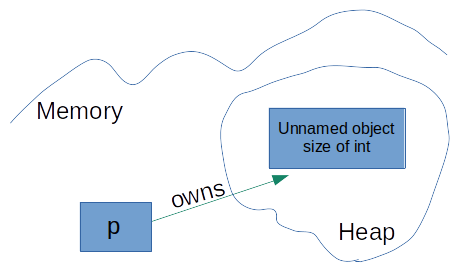
\includegraphics[width=1\textwidth, height=1\textheight, keepaspectratio]{./imgs/unique_ptr_definition.png}
	\caption{Unique ptr}
	\label{fig:unique_ptr_definition}
\end{figure}

\textsf{\small Se lo \textbf{unique\_ptr} viene distrutto, anche la memoria allocata nell'heap viene distrutta di conseguenza.} \\

\begin{figure}[H]
	\centering
	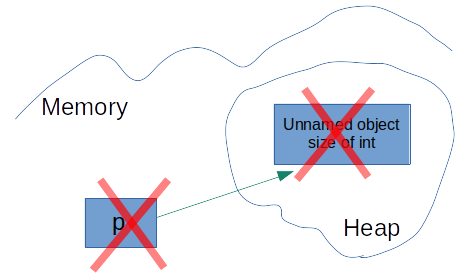
\includegraphics[width=1\textwidth, height=1\textheight, keepaspectratio]{./imgs/unique_ptr_delete.png}
	\caption{Unique ptr delete}
	\label{fig:unique_ptr_delete}
\end{figure}

\textsf{\small Per creare uno \textbf{unique\_ptr} si può anche utilizzare \textbf{std::make\_unique}.} \\

\begin{lstlisting}
	#include <iostream>
	
	class Rectangle {
		public:
			Rectangle(int w, int h)
			{
				this->width = w;
				this->height = h;
			}
		
			int area()
			{
				return width * height;
			}
		
		private:
			int width;
			int height;
	};

	int main()
	{
		auto pRect = std::make_unique<Rectangle>(3, 4);
		std::cout << "Area del rettangolo: " << pRect->area() << std::endl; //Output: Area del rettangolo: 12
		return 0;
	}
\end{lstlisting}

\subsubsection{Differenza tra std::make\_unique vs std::unique\_ptr}

\textsf{\small Ci sono varie ragioni per cui utilizzare \textbf{std::make\_unique} al posto di \textbf{std::unique\_ptr} con la new: } \\

\begin{itemize}
	\item \textsf{\small È sicuro nel caso si vogliano creare dei temporanei, mentre con la new ti devi ricordare la regola: del non usare temporanei senza nome. } 
	\item \textsf{\small Con l'utilizzo di \textbf{make\_unique} si può finalmente evitare di usare la \textbf{new}, a differenza della vecchia regola: mai usare la \textbf{new} tranne per gli \textbf{unique\_ptr}.} 
	\item \textsf{\small Non richiede \emph{type usage} ridondante: \emph{unique\_ptr<T>(new T())} -> make\_unique<T>().} \\
	\item \textsf{\small Così da non dover esplicitare gli argomenti dei \emph{template types}.}
	\item \textsf{\small Aggiunge sicurezza riguardo le eccezioni.}
	\item \textsf{\small Altrimenti non potresti accedere al costruttore della classe fuori dallo \emph{scope} corrente.}
	%\item \textsf{\small }
\end{itemize}

\subsubsection{Ownership | move}

\textsf{\small Un \textbf{unique pointer} è una relazione 1 a 1 con l'oggetto allocato.} \\

\textsf{\small Non può essere copiato o passato per valore, però la \textbf{ownership} (proprietà) dell'oggetto può essere trasferita.} \\

\begin{lstlisting}
	#include <iostream>
	
	class Person {
		public:
			Person(std::string s) : name(s) {};
			~Person() { std::cout << "Libero spazio" << std::endl };
			
			std::string getName() { return this->name };
			
		private:
			std::string name;
	};

	int main()
	{
		auto ptrPerson = std::make_unique<Person>("Luigi");
		
		std::cout << "Nome: " << ptrPerson->getName() << std::endl; //Output: Nome: Luigi
		
		std::unique_ptr<Person> ptrPerson2;
		
		ptrPerson2 = std::move(ptrPerson);
		
		std::cout << "Nome: " << ptrPerson2->getName() << std::endl; //Output: Nome: Luigi
		
		std::cout << "Nome dopo il trasferimento dell'ownership: " << ptrPerson->getName() << std::endl; //Output: [non stampa niente]
		
		return 0;
	}
\end{lstlisting}

\begin{figure}[H]
	\centering
	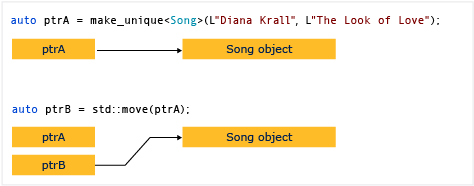
\includegraphics[width=1\textwidth, height=1\textheight, keepaspectratio]{./imgs/unique_ptr_move2.png}
	\caption{Unique ptr move}
	\label{fig:unique_ptr_move2}
\end{figure}

\subsubsection{Operazioni sugli unique\_ptr}

\textsf{\small Varie operazioni sono supportate sugli \textbf{unique\_ptr}: } \\

\begin{itemize}
	\item \textsf{\small \textbf{*} : Dereferenza del puntatore.}
	\item \textsf{\small \textbf{->} : Accedere ai membri della classe.}
	\item \textsf{\small \textbf{.get()} : per ottenere il \emph{raw pointer} del \textbf{unique\_ptr} (non cancellarlo, perché è gestito dal unique pointer; è da usare solo per calcoli).}
	\item \textsf{\small \textbf{.reset(new int())} : cancella il vecchio oggetto e ne crea uno nuovo (al posto di new int() avremmo potuto passare qualsiasi altro oggetto, era per fare un esempio).}
	\item \textsf{\small \textbf{move} : trasferisce la proprietà del \textbf{unique\_ptr}.}
	\item \textsf{\small \textbf{swap} : per scambiare due \textbf{unique pointers}.}
	\item \textsf{\small \textbf{if(unique\_ptr)} : se passiamo uno \textbf{unique\_ptr} all'if, questo restituisce falso se non è associato a nessun oggetto.}
	%\item \textsf{\small \textbf{} : }
\end{itemize}

\subsubsection{Passare uno unique\_ptr ad una funzione}

\textsf{\small Utilizziamo \textbf{std::move} per trasferire la proprietà del \textbf{unique\_ptr}.} \\

\begin{lstlisting}
	#include <iostream>
	#include<memory>
	
	struct A {
		int x;
		~A() { std::cout << "Libero spazio" << std::endl };
	};

	void passUniquePtr(std::unique_ptr<A> a)
	{
		// Usciti dalla funzione, lo unique\_ptr e il suo oggetto vengono cancellati, perché locali alla funzione.
		std::cout << "Puntatore ricevuto" << '\n';
		a->x = 5;
		std::cout << "a.x: " << a->x << std::endl;
	}

	int main()
	{
		auto ptrA = std::make_unique<A>();
		passUniquePtr(std::move(ptrA));
		
		// true = ptrA è vuoto.
		if(!ptrA)
		{
			std::cout << "ptrA è vuoto" << std::endl;
		}
	
		//Output: Puntatore ricevuto
		//Output: a.x: 5
		//Output: Libero spazio
		//Output: ptrA è vuoto
		return 0;
	}
\end{lstlisting} 

\subsubsection{Restituire un unique\_ptr}

\textsf{\small Si può restituire uno \textbf{unique\_ptr} da una funzione. } \\

\begin{lstlisting}
	#include <iostream>
	#include <memory>
	
	class A {};
	
	std::unique_ptr<A> returnUniquePtr()
	{
		auto a = std::make_unique<A>();
		return a;
	}

	int main()
	{
		auto ptrA = returnUniquePtr();
		
		if(ptrA)
		{
			std::cout << "ptrA ha un oggetto. " << std::endl;	
		}
	
		//Output: ptrA ha un oggetto.
		return 0;
	}
\end{lstlisting}

\subsubsection{Membri delle classi: unique pointer vs raw pointer vs reference}

\textsf{\small } \\

\begin{itemize}
	\item \textsf{\small \textbf{Unique pointer membro della classe} : la classe è la proprietaria dell'oggetto del puntatore.}
	\item \textsf{\small \textbf{Raw pointer membro della classe} : La classe è un osservatore e non è responsabile di rimuovere l'oggetto puntato dal puntatore. Viene rimosso da uno smart pointer fuori dalla classe.}
	\item \textsf{\small \textbf{Referenza membro della classe} : è garantito che la referenza contiene dati validi mentre la classe è "viva".}
	%\item \textsf{\small }
\end{itemize}

\subsection{share pointers}

\textsf{\small \textbf{Definizione: } Gli \textbf{shared pointers} sono un tipo di \textbf{smart pointers} dove più di un puntatore può puntare allo stesso oggetto e un contatore (\emph{Reference Counter}) verrà mantenuto di conseguenza.} \\

\textsf{\small Abbiamo sempre bisogno di includere l'header \textbf{<memory>} per poterlo utilizzare.} \break

\begin{lstlisting}
	#include <iostream>
	#include <memory>
	
	class A {
		public:
			int x;
			A(int x) : x(x){};
	};

	int main()
	{
		auto sharedPtr1 = std::make_shared<A>(7); // oppure si può anche fare: std::shared\_ptr<A> sharedPtr1(new A{7});
		
		std::shared_ptr<A> sharedPtr2 = sharedPtr1;
		std::shared_ptr<A> sharedPtr3 = sharedPtr1;
		
		// Tutti e tre gli \textbf{shared1\_ptr} puntano allo stesso oggetto.
		return 0;
	}
\end{lstlisting}

\newpage %TODO: questo \newpage mi serviva per evitare gli spazi bianchi sopra la subsection share pointers.

\begin{figure}[H]
	\centering
	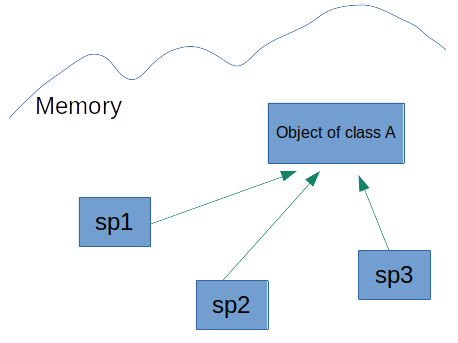
\includegraphics[width=1\textwidth, height=1\textheight, keepaspectratio]{./imgs/shared_ptr3.png}
	\caption{Shared ptr}
	\label{fig:shared_ptr3}
\end{figure}

\textsf{\small Possiamo creare uno \textbf{shared pointer} sia con \textbf{shared\_ptr} sia con \textbf{make\_shared}.} \\

\subsubsection{Differenza tra std::shared\_ptr vs std::make\_shared}

\textsf{\small Una delle differenze tra questi due è che \textbf{make\_shared} performa una sola allocazione nell'heap, mentre \textbf{shared\_ptr} ne fa due.} \\

\textsf{\small \textbf{shared\_ptr} si occupa di due entità: } \\

\begin{itemize}
	\item \textsf{\small Il blocco di controllo (\emph{control block}) che memorizza dei metadati come \emph{ref-counts} (contatore delle referenze all'oggetto), \emph{type-erased deleter}, ecc.}
	\item \textsf{\small l'oggetto stesso.}
\end{itemize}

\textsf{\small \textbf{std::make\_shared} fa una singola allocazione nell'heap per lo spazio necessario sia per il \emph{control block} sia per \emph{l'oggetto}. } \break

\textsf{\small Inoltre \textbf{std::make\_shared} è \emph{exception-safe} (sicuro per quanto riguarda le eccezioni).} \\

\textsf{\small Per di più, \textbf{make\_shared} sfrutta dell'ottimizzazione conosciuta come \emph{We know Where You Live} che permette al \emph{control block} di essere un piccolo puntatore, quindi \textbf{make\_shared} non solo evita un'ulteriore allocazione, ma alloca anche meno memoria totale.} \break

\textsf{\small Un problema che potrebbe esserci per quanto riguarda \textbf{std::make\_shared} è che visto che fa una singola allocazione, non c'è modo di deallocare la memoria del \emph{control block} e dell'\emph{oggetto} in modo indipendente. Un altro svantaggio, di conseguenza è che essendoci una singola allocazione, la memoria non può essere deallocata finché il \emph{control block} non è più usato. } \\

\subsubsection{Operazioni sui shared pointers}

\textsf{\small Sono possibili varie operazioni sugli \textbf{shared pointers}: } \\

\begin{itemize}
	\item \textsf{\small \textbf{(*nomepuntatore).variabile} : dereferenza}
	\item \textsf{\small \textbf{nomepuntatore->variabile} : dereferenza come sopra}
	\item \textsf{\small \textbf{.get()} : per poter accedere al \emph{raw pointer} chiamato \textbf{stored pointer}.}
	\item \textsf{\small \textbf{use\_count()} : per ottenere il numero di \textbf{shared\_ptr} che puntano allo stesso oggetto.}
	\item \textsf{\small \textbf{.reset()} : scollega e svuota il puntatore.}
\end{itemize}

\textsf{\small Lo \textbf{shared pointer} inoltre allo \emph{stored pointer}, possiede un secondo puntatore che punta ad un \textbf{control block}. Il \emph{control block} ha un \emph{reference counter} (contatore delle referenze) che memorizza il numero di \textbf{shared pointers} che puntano allo stesso oggetto.} \\

\newpage %TODO: questo mi serviva per evitare gli spazi nell'itemize della subsubsection "Operazioni sui shared pointers".

\begin{figure}[H]
	\centering
	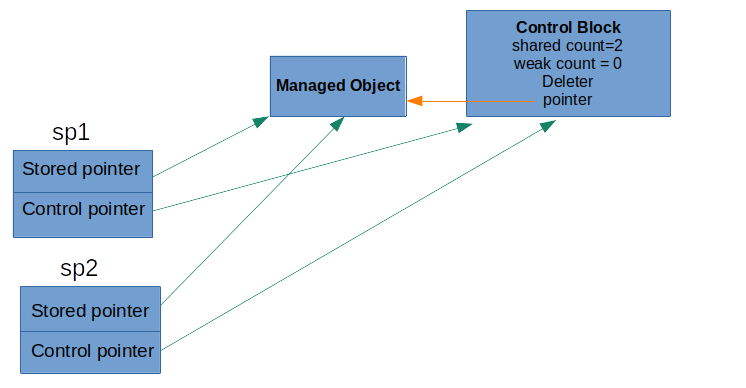
\includegraphics[width=1\textwidth, height=1\textheight, keepaspectratio]{./imgs/shared_ptr_structure.png}
	\caption{Shared ptr structure}
	\label{fig:shared_ptr_structure}
\end{figure}

\subsubsection{Distruzione degli shared pointers}

\textsf{\small Quando verrà eliminato l'oggetto gestito dagli \textbf{shared\_ptr}?} \\

\textsf{\small Quando uno \textbf{shared pointer} viene distrutto, allora il \emph{control block} decrementerà il \emph{reference counter}.} \\

\textsf{\small L'oggetto verrà eliminato quando l'ultimo \textbf{shared\_ptr} verrà eliminato. (e quindi quando il \emph{reference counter} arriverà a 0. )} \\

\begin{lstlisting}
	#include <iostream>
	#include <memory>
	
	class A {
		public:
			int x;
			A(int x) : x(x) {};
	};

	int main()
	{
		auto shrPtr1 = std::make_shared<A>(5);
		auto shrPtr2 = shrPtr1;
		auto shrPtr3 = shrPtr1;
		
		{
			auto shrPtr4 = shrPtr1;
			std::cout << shrPtr1.use_count() << std::endl; //Output: 4
		}
		
		std::cout << shrPtr1.use_count() << std::endl; //Output: 3
		
		shrPtr3 = std::make_shared<A>(8); // shrPtr3 punta ad un altro oggetto.x
		
		shrPtr2.reset(); // shrPtr2 scollegato e svuotato.
		
		std::cout << shrPtr1.use_count() << std::endl; //Output: 1
		return 0;
	}
\end{lstlisting}

\begin{figure}[H]
	\centering
	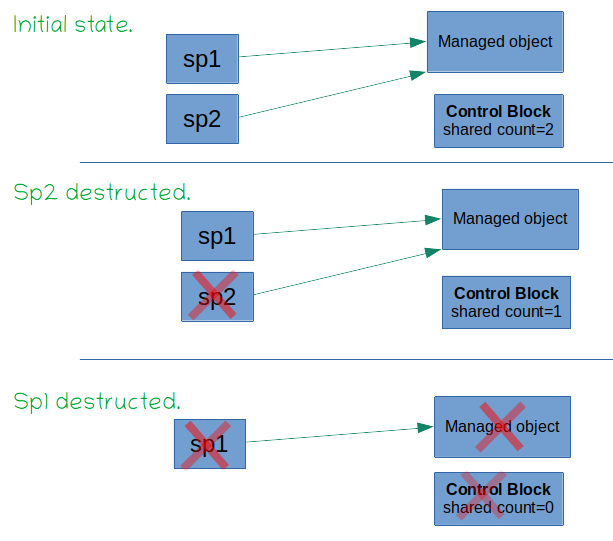
\includegraphics[width=1\textwidth, height=1\textheight, keepaspectratio]{./imgs/shared_ptr_destruction.png}
	\caption{Shared ptr destruction}
	\label{fig:shared_ptr_destruction}
\end{figure}

\subsubsection{Passare gli shared pointers ad una funzione}

\textsf{\small Se una funzione vuole l'\emph{ownership} (proprietà) su un \textbf{shared\_ptr}, possiamo passarlo per valore: } \\

\begin{lstlisting}
	#include <iostream>
	#include <memory>
	
	void function(std::shared_ptr<int> sp)
	{
		std::cout << sp.use_count() << std::endl;
	}

	int main()
	{
		auto sp1 = std::make_shared<int>(6);
		std::cout << sp1.use_count() << std::endl; //Output: 1
		
		function(sp1); //Output: 2
		
		std::cout << sp1.use_count() << std::endl; //Output: 1 (lo shared\_ptr nella funzione "function" viene distrutto una volta usciti da essa, perché è locale alla funzione)
		return 0;
	}
\end{lstlisting}

\subsubsection{Restituire gli shared pointers}

\textsf{\small Una funzione può restituire \textbf{shared\_ptr} per valore: } \\

\begin{lstlisting}
	#include <iostream>
	#include <memory>
	
	std::shared_ptr<int> function()
	{
		auto sp = std::make_shared<int>(9);
		return sp;
	}

	int main()
	{
		auto sp1 = function(); // Lo shared\_ptr dentro alla funzione non esiste più, però viene ritornato e recuperato nella variabile sp1.
		
		std::cout << sp1.use_count() << std::endl; //Output: 1
		std::cout << *sp1 << std::endl; //Output: 9
		return 0;
	}
\end{lstlisting}

\textsf{\small Un problema col restituire uno \textbf{shared\_ptr}: se lo devi restituire al "mondo esterno", meglio restituirlo come \emph{reference}, perché altrimenti uno potrebbe chiamare la \textbf{.reset()} su quello \textbf{shared pointer}.} \break %TODO: ma non potrebbero comunque chiamarla la .reset() anche con la reference?

\textsf{\small Un altro modo per restituire uno \textbf{shared\_ptr} è attraverso \emph{std::allocate\_shared}.} \\

\begin{lstlisting}
	#include <iostream>
	#include <memory>
	
	int main () {
		std::allocator<int> alloc;    // allocatore di default per gli int.
		std::default_delete<int> del; // deleter di default per gli int.
		
		std::shared_ptr<int> foo = std::allocate_shared<int> (alloc,12);
		
		auto bar = std::allocate_shared<int> (alloc,24);
		
		auto baz = std::allocate_shared<std::pair<int,int>> (alloc,33,44);
		
		std::cout << "*foo: " << *foo << '\n'; //Output: *foo: 12
		std::cout << "*bar: " << *bar << '\n'; //Output: *bar: 24
		std::cout << "*baz: " << baz->first << ' ' << baz->second << '\n'; //Output: *baz: 33 44
		
		return 0;
	}
\end{lstlisting}

\subsubsection{static\_pointer\_cast}

\textsf{\small \textbf{Definizione: } \textbf{static\_pointer\_cast} è una funzione, non una keyword e restituisce uno \textbf{shared\_ptr} che possiede e contiene un puntatore all'oggetto costruito.} \\

\textsf{\small Se il parametro passato non è vuoto, ciò che viene restituito condivide la proprietà con il parametro passato, quindi il contatore viene incrementato di 1.} \\

\textsf{\small Se il parametro è vuoto (non possiede nulla), allora l'oggetto ritornato è uno \textbf{shared\_ptr} vuoto.} \\

\begin{lstlisting}
	#include <iostream>
	#include <memory>
	
	class Base {};
	
	class Derived : public Base {
		public:
			void print()
			{
				std::cout << "Hello World!" << std::endl;
			}
	};

	int main()
	{
		std::shared_ptr<Base> spBase(std::make_shared<Derived>());
		
		std::static_pointer_cast<Derived>(spBase)->print();
		
		static_cast<Derived*>(spBase.get())->print();
		
		//Output: Hello World!
		//Output: Hello World!
		return 0;
	}
\end{lstlisting}

\begin{figure}[H]
	\centering
	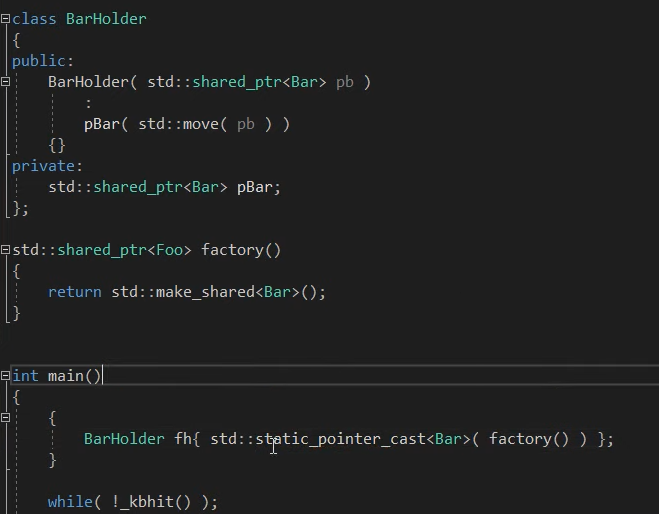
\includegraphics[width=1\textwidth, height=1\textheight, keepaspectratio]{./imgs/std_shared_ptr_std_static_pointer_cast2.png}
	\caption{Static pointer cast}
	\label{fig:std_shared_ptr_std_static_pointer_cast2}
\end{figure}

%TODO: dynamic_pointer_cast (volendo, ma non necessario, giusto per approfondimento)
%TODO: const_pointer_cast

\subsubsection{enable\_shared\_from\_this}

\textsf{\small \textbf{Definizione: } \textbf{std::enable\_shared\_from\_this} permette a un oggetto \emph{t} che è gestito da uno \textbf{shared\_ptr} \emph{sp} di generare, in modo sicuro, degli \textbf{shared\_ptr} addizionali, istanze \emph{sp1}, \emph{sp2} che condividono tutti la proprietà dell'oggetto \emph{t} con \emph{sp}.} \break

\textsf{\small Ereditare da \textbf{std::enable\_shared\_from\_this} fornisce il tipo T con una funzione membro \emph{shared\_from\_this()}. Se un oggetto \emph{t} di tipo T è gestito da uno \textbf{shared\_ptr} \emph{sp}, allora chiamare \emph{shared\_from\_this()} restituirà un nuovo \textbf{shared\_ptr} che condivide la proprietà di \emph{t} con \emph{sp}. } \\

\begin{lstlisting}
	#include <iostream>
	#include <memory>
	
	struct B : std::enable_shared_from_this<B> {};
	
	int main()
	{
		std::shared_ptr<B> foo, bar;
		
		foo = std::make_shared<B>();
		
		bar = foo->shared_from_this();
		
		if(!foo.owner_before(bar) && !bar.owner_before(foo))
		{
			std::cout << "foo e bar condividono la proprietà" << std::endl;
		}
	
		//Output: foo e bar condividono la proprietà
	
		return 0;
	}
\end{lstlisting}

\textsf{\small Inoltre, c'è anche una funzione \emph{weak\_from\_this} che restituisce un \textbf{weak\_ptr} che tiene traccia della proprietà di \textbf{*this} da parte di tutte le istanze di \textbf{shared\_ptr}.} \\

\subsubsection{Performance degli shared pointers}

\textsf{\small Uno \textbf{shared pointer} ha bisogno di due \emph{raw pointers}. Un insieme di \textbf{shared pointers} hanno bisogno di essere gestiti da una \emph{control unit} (\emph{control block}). Quindi la memoria che uno \textbf{shared pointer} occupa è maggiore dei \emph{raw} e degli \textbf{unique} pointers.} \\

\subsubsection{Shared pointers, unique pointers or raw pointers}

\textsf{\small Se un oggetto ha bisogno di un singolo proprietario per tutta la durata del programma e possiamo immaginare il puntatore come un'entità singola, allora usiamo un \textbf{unique pointer}. Per delle performance più buone gli \textbf{unique pointers} sono migliori rispetto agli \textbf{shared pointers}.} \\

\textsf{\small Gli \textbf{shared pointers} sono utili dove non abbiamo bisogno di pensare alle \emph{performance}, \emph{ownership} e \emph{lifetime} degli oggetti.}

\subsection{weak pointers}

\textsf{\small \textbf{Definizione: } Un \textbf{weak pointer} è un tipo di \textbf{smart pointer} che non prende la proprietà dell'oggetto, ma agisce come un osservatore. Non partecipa al \emph{reference counter} (non viene contato) e non estende la \emph{lifetime} dell'oggetto. } \break 
\textsf{\small Sono usati, principalmente, per rompere la dipendenza circolare degli \textbf{shared pointers}.} \\

\subsubsection{Problema della dipendenza ciclica}

\textsf{\small \textbf{Definizione: } Mettiamo di avere due classi: A e B, se entrambe hanno un puntatore che punta all'altra, avremo un ciclo e il \emph{use\_count()} non arriverà mai a 0, il che creerebbe un problema nella rimozione di questi due puntatori.} \\

\begin{figure}[H]
	\centering
	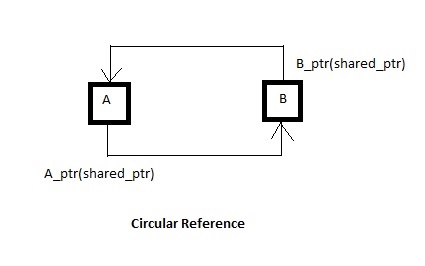
\includegraphics[width=1\textwidth, height=1\textheight, keepaspectratio]{./imgs/shared_ptr_problem_cyclic_dependency.jpg}
	\caption{Cyclic dependency}
	\label{fig:shared_ptr_problem_cyclic_dependency}
\end{figure}

\textsf{\small Per questo motivo usiamo gli \textbf{weak pointers}, perché non vengono conteggiati nel \emph{reference counter}. Possono, comunque avere accesso all'oggetto.} \\

\begin{figure}[H]
	\centering
	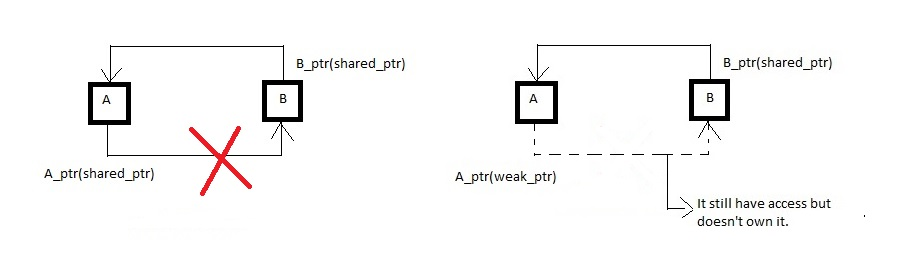
\includegraphics[width=1\textwidth, height=1\textheight, keepaspectratio]{./imgs/shared_ptr_problem_cyclic_dependency2.jpg}
	\caption{Cyclic dependency}
	\label{fig:shared_ptr_problem_cyclic_dependency2}
\end{figure}

\textsf{\small Quindi, il problema della \emph{dipendenza ciclica} si risolve con l'utilizzo degli \textbf{weak pointers}.} \\

\subsubsection{Quando usare i weak pointers?}

\textsf{\small \textbf{Quando usare i weak pointers?}} \break

\textsf{\small Quando vuoi riferire al tuo oggetto da molteplici posti, per quelle referenze dove non è okay ignorarle e deallocarle.} \\

%TODO: risolvere problema del danglin pointer

\subsubsection{Operazioni sugli weak pointers}

\textsf{\small Ci sono varie operazioni sui \textbf{weak pointers}: } \\

\begin{itemize}
	\item \textsf{\small \textbf{*} : dereferenza}
	\item \textsf{\small \textbf{->} : dereferenza, accedere ai membri della classe/struct, ecc.}
	\item \textsf{\small \textbf{.lock()} : restituisce uno \textbf{shared\_ptr} con le informazioni preservate nel \textbf{weak\_ptr} se non è \emph{expired}. Se il \textbf{weak\_ptr} è \emph{expired} (scaduto), la funzione restituisce un \textbf{shared\_ptr} vuoto.}
	%\item \textsf{\small \textbf{.get()} : }
	\item \textsf{\small \textbf{.reset()} : cancella il vecchio oggetto e ne crea uno nuovo.}
	\item \textsf{\small \textbf{.swap()} : scambia due \textbf{weak pointers}.}
	\item \textsf{\small \textbf{.use\_count()} : restituisce il numero di \textbf{shared pointers} che puntano allo stesso oggetto.}
	\item \textsf{\small \textbf{.expired()} : restituisce se il \textbf{weak\_ptr} è vuoto o non ci sono più \textbf{shared\_ptr} nell' \emph{owner group}. I puntatori "scaduti" (\emph{expired}) sono come \textbf{weak pointers} vuoti quando \emph{locked} e non possono quindi essere più usati.}
	\item \textsf{\small \textbf{.owner-before()} : restituisce se l'oggetto deve andare prima del parametro. Se l'oggetto appartiene allo stesso \emph{owner group} del parametro, allora restituisce \emph{false}, anche se il valore memorizzato dai puntatori è diverso.}
	%\item \textsf{\small \textbf{} : }
\end{itemize}

\begin{lstlisting}
	#include <iostream>
	#include <memory>
	
	class Person {
		public:
			std::string name;
			Person(std::string name) : name(name){};
	};
	
	int main()
	{
		std::weak_ptr<Person> wp;
		
		auto teacher = std::make_shared<Person>("Giorgio");
		
		wp = teacher;
		
		// Per controllare se l'oggetto è ancora lì o no.
		// lock() restituisce un shared\_ptr temporaneo.
		if(auto temp = wp.lock())
		{
			std::cout << temp->name << std::endl;
		} else {
			std::cout << "L'oggetto non c'è più" << std::endl;
		}
		return 0;
	}
\end{lstlisting}

\newpage %TODO: questo \newpage mi serviva per gli spazi bianchi.

\begin{figure}[H]
	\centering
	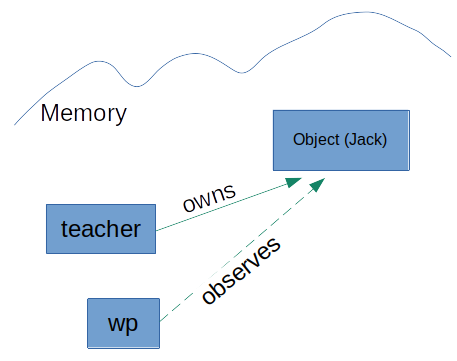
\includegraphics[width=1\textwidth, height=1\textheight, keepaspectratio]{./imgs/weak_ptr1.png}
	\caption{Weak pointers}
	\label{fig:weak_ptr1}
\end{figure}

\textsf{\small Uno \textbf{shared pointer} ha un \textbf{control block} che conta il numero di \textbf{shared pointers} e di \textbf{weak pointers}. Quando il contatore degli \textbf{shared pointers} arriva a 0, l'oggetto viene eliminato, ma il \emph{control block} resta vivo finché il contatore dei \textbf{weak pointers} non raggiunge 0.} \\

% -------------------------- SECTION: COPY-AND-SWAP IDIOM ----------------------------

\section{Copy-And-Swap Idiom}

\textsf{\small \textbf{Cos'è il \textbf{copy-and-swap idiom} e a cosa serve?}} \break

\textsf{\small Qualsiasi classe che gestisce una risorsa (\emph{un wrapper}, come uno \textbf{smart pointer}) ha bisogno di implementare la \emph{Rule of Three} (destructor, copy constructor, copy assignment). La \emph{copy-and-swap} assiste il \emph{copy assignment} in due cose: evitare la duplicazione di codice e fornisce una forte sicurezza a livello di eccezioni (\emph{exception safety}).} \\

\textsf{\small Concettualmente funziona utilizzando la funzionalità del \emph{copy constructor} di creare una copia locale dei dati, prendere questa copia con una funzione \emph{swap}, scambiando i vecchi dati con quelli nuovi.} \\

\textsf{\small La copia temporanea viene distrutta, portandosi i vecchi dati con essa. Restiamo con una copia dei nuovi dati.} \\

\textsf{\small Per poter far questo quindi avremo bisogno di: } \\

\begin{itemize}
	\item \textsf{\small copy-constructor}
	\item \textsf{\small destructor}
	\item \textsf{\small swap function}
\end{itemize}

\begin{lstlisting}
	#include <iostream>
	#include <cstring>
	
	class anyArrayClass
	{
		int size;
		int *ptr;
		public:
		anyArrayClass(int s=0):size(s),
		ptr(size ? new int[size]:nullptr) {}
		
		// Copy constructor
		anyArrayClass(const anyArrayClass& obj):size(obj.size),
		ptr(size ? new int[size]:nullptr)
		{
			memmove(ptr, obj.ptr, size*sizeof(int));
		}
		
		friend void swap(anyArrayClass& obj1, anyArrayClass& obj2)
		{
			std::swap(obj1.size, obj2.size);
			std::swap(obj1.ptr, obj2.ptr);
		}
		
		// overloaded assignment operator
		// argomento passato per valore. chiama il copy constructor
		anyArrayClass& operator=(anyArrayClass obj)	
		{
			// calling friend function
			swap(*this, obj);
			return *this;
		}
		
		~anyArrayClass()
		{
			delete[] ptr;
		}
	};
\end{lstlisting}

\textsf{\small I vantaggi sono: } \\

\begin{itemize} %TODO: questo è da riguardare.
	\item \textsf{\small Non c'è più bisogno di controlli per l'assegnamento a se stesso visto che il parametro è passato per valore. Inoltre l'allocazione a se stesso è molto rara quindi l'\emph{overhead} della copiatura non dovrebbe essere un problema.}
	\item \textsf{\small Ora il \emph{copy constructor} è usato per creare un oggetto temporaneo, lo swapping (scambio) avverrà soltanto se l'oggetto temporaneo è stato creato affatto. Praticamente, quello che stiamo facendo manualmente, il compilatore lo sta facendo per noi.}
	\item \textsf{\small Riusabilità del codice: l'operatore \emph{operator=()} non ha molto codice nel suo corpo, anzi stiamo usando il \emph{copy constructor} e la funzione \emph{swap} per fare il lavoro.}
\end{itemize}

%\textsf{\small \textbf{Nota:} Non puoi usare \textbf{std::swap} visto che internamente usa il \emph{copy constructor} e l'\emph{assignment operator}.} \\ %TODO: c'è bisogno di ulteriori verifiche.

% ---------------------- SECTION: TECNICHE PER IL DEBUGGING --------------------------

\newpage

\section{Tecniche per il debugging}

\textsf{\small \textbf{Definizione: } \textbf{Debugging} si riferisce alle tecniche impiegate dai programmatori per cercare di correggere gli errori, i bugs di un programma.} \\

\textsf{\small Una metodologia di base è questa: } \\

\begin{itemize}
	\item \textsf{\small Osservare il problema.}
	\item \textsf{\small Identificare la natura del problema.}
	\item \textsf{\small Identificare la condizione (o condizioni) che innesca il problema.}
	\item \textsf{\small Identificare il meccanismo di guasto, fallimento.}
	\item \textsf{\small Fixare il problema.}
	%\item \textsf{\small }
\end{itemize}

\textsf{\small Per fare questo potrebbe tornare utile: } \\

\begin{itemize}
	\item \textsf{\small Commentare il codice.}
	\item \textsf{\small Validare il flusso del codice, programma (\emph{code flow}).}
	\item \textsf{\small Controllare valori stampandoli a schermo.}
\end{itemize}

%TODO: magari approfondire, puù degli esempi

% ---------------------- SECTION: DEPENDENCY INJECTION -------------------------------

%TODO: pattern? Magari in un capitolo sui Design Patterns

%\newpage

%\section{Dependency Injection}

%\textsf{\small \textbf{Definizione: } } \\

% ---------------------- SECTION: POINTER TO FUNCTION --------------------------------

\newpage

\section{Puntatore a funzione}

\textsf{\small \textbf{Definizione: } I \textbf{puntatori a funzione} o \textbf{function pointers} sono dei puntatori che puntano a delle funzioni.} \\ %TODO: la definizione è da: "grazie al cazzo".

\begin{lstlisting}
	#include <iostream>
	
	void fun(int a)
	{
		std::cout << "Valore di a: " << a << std::endl;
	}
	
	int main()
	{
		// fun\_ptr è un puntatore alla funzione fun() (quella sopra)
		void (*fun_ptr)(int) = &fun;
		
		/* La riga sopra è equivalente alle seguenti due sotto:
		void (*fun_ptr)(int);
		fun_ptr = &fun;
		*/
		
		// Chiamando fun() attraverso fun\_ptr
		(*fun_ptr)(10);
		
		return 0;
	}
\end{lstlisting}

\textsf{\small Si può anche scrivere così: } \\

\begin{lstlisting}
	#include <iostream>
	
	void fun(int a)
	{
		std::cout << "Il valore di a: " << a << std::endl;
	}
	
	int main()
	{
		void (*fun_ptr)(int) = fun; // \& rimosso
		
		fun_ptr(10); // * rimosso
		
		return 0;
	}
\end{lstlisting}

\textsf{\small Alcuni fatti riguardo i \textbf{function pointers} dal C: } \\

\begin{itemize}
	\item \textsf{\small Questi puntano all'inizio del codice eseguibile.}
	\item \textsf{\small A differenza dei normali puntatori, non allochiamo e deallochiamo memoria usando i \textbf{function pointers}.}
	\item \textsf{\small Il nome della funzione può anche essere usato per ottenere l'indirizzo della funzione.}
	\item \textsf{\small Proprio come i puntatori normali, possiamo avere un array di \textbf{function pointers}.}
	\item \textsf{\small Possono essere usati al posto degli switch.}
	\item \textsf{\small Come i puntatori normali anche questi possono essere passati come argomenti e restituiti dalle funzioni.}
	\item \textsf{\small Alcune funzionalità del C++ sono implementate usando i \textbf{function pointers}, come ad esempio le \textbf{funzioni virtuali}.}
\end{itemize}

\begin{lstlisting}
	#include <iostream>
	
	void add(int a, int b)
	{
		std::cout << "Addizione: " << a + b << std::endl;
	}
	void subtract(int a, int b)
	{
		std::cout << "Sottrazione: " << a - b << std::endl;
	}
	void multiply(int a, int b)
	{
		std::cout << "Moltiplicazione: " << a * b << std::endl;
	}
	
	int main()
	{
		// fun\_ptr\_arr è un array di function pointers (puntatori a funzioni).
		void (*fun_ptr_arr[])(int, int) = {add, subtract, multiply};
		unsigned int ch, a = 7, b = 5;
		
		printf("Enter Choice: 0 for add, 1 for subtract and 2 "
		"for multiply\n");
		std::cout << "0. Aggiungi" << "\n";
		std::cout << "1. Riduzione" << "\n";
		std::cout << "2. Moltiplicazione" << "\n";
		std::cout << "Scelta: ";
		
		std::cin >> ch;
		
		if (ch > 2) return 0;
		
		(*fun_ptr_arr[ch])(a, b);
		
		return 0;
	}
\end{lstlisting}

%TODO: std::function

% -------------------------- SECTION: 7 CONCETTI AVANZATI ----------------------------

\newpage

%TODO: Questo come ultimo argomento del capitolo!

\section{7 Concetti Avanzati}

\begin{figure}[H]
	\centering
	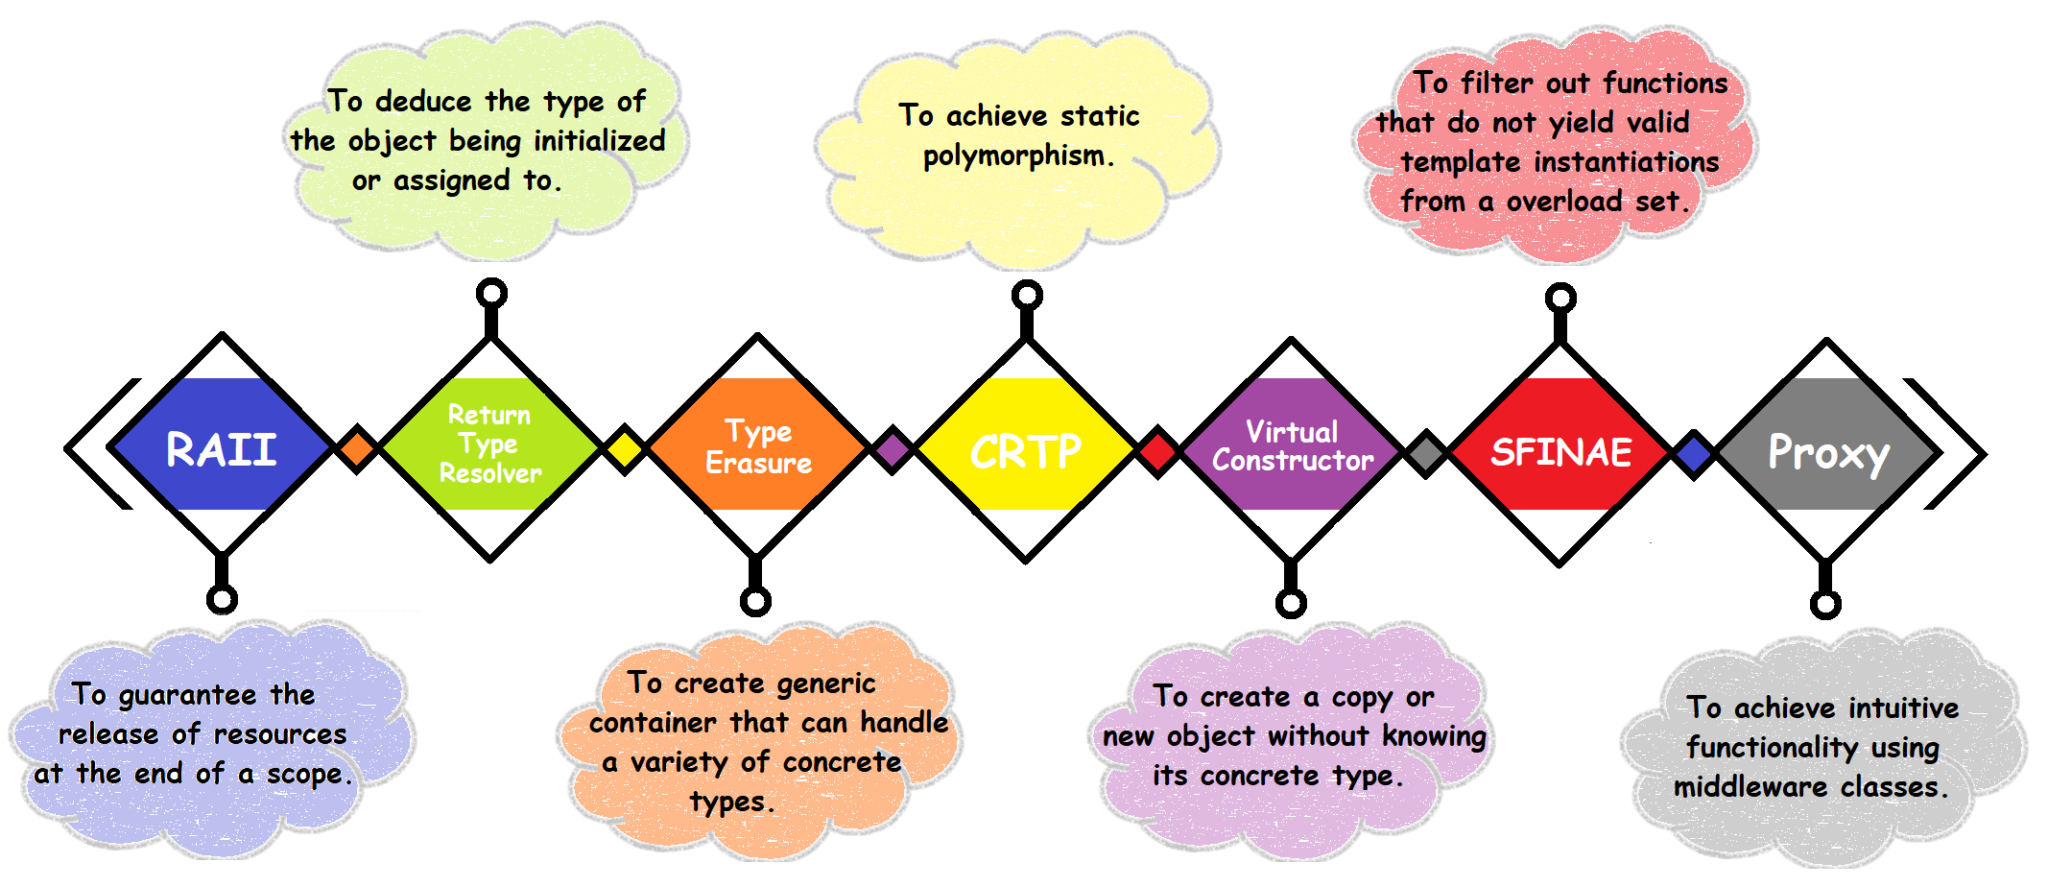
\includegraphics[width=1\textwidth, height=1\textheight, keepaspectratio]{./imgs/7-Advanced-C-programming-styles-and-idiom-examples-you-should-know.png}
	\caption{7 Concetti Avanzati}
	\label{fig:7-Advanced-C-programming-styles-and-idiom-examples-you-should-know}
\end{figure}

\subsection{RAII}

\textsf{\small Abbiamo già trattato questo argomento nel precedente capitolo \emph{Concetti Intermedi}, ma lo riprenderemo qui visto che è uno dei 7 Concetti Avanzati del linguaggio.} \\

\textsf{\small \textbf{Definizione: } \textbf{RAII} (\emph{\textbf{R}esource \textbf{A}cquisition \textbf{i}s \textbf{I}nitialization}), o anche conosciuta come \emph{Execute-around object}, \emph{Resource release is finalization}, \emph{Scope-bound resource management} è una tecnica di programmazione il cui intento è quello di rilasciare le risorse precedentemente allocate alla fine dello scope. } \\

\textsf{\small Implementiamo questo attraverso: il \emph{wrapping} delle risorse nella classe; acquisizione della risorse nel costruttore immediatamente dopo l'allocazione e automaticamente rilasciata nel distruttore; risorse usate attraverso un'interfaccia della classe.} \\

\begin{lstlisting}
	#include <iostream>
	
	class Resource {
		public:
			Resource(int x, int y) { std::cout << "risorsa acquisista\n"; }
			~Resource() { std::cout << "risorsa distrutta\n"; }
	};

	void func()
	{
		Resource *ptr = new Resource(1, 2);
		int x;
		
		std::cout << "Inserisci un numero: ";
		std::cin >> x;
		
		if(x == 0)
		{
			// La funzione restituisce prima del return e quindi ptr non verrà deallocato, cancellato!
			throw 0;
		} else if(x < 0) {
			// La funzione restituisce prima della deallocazione, quindi ptr non verrà deallocato!
			return;
		}
		delete ptr;
	}

	int main()
	{
		func();
		return 0;
	}
\end{lstlisting}

\textsf{\small Nel codice sopra, il \emph{return} o il \emph{throw} avvengono prima della \textbf{delete} quindi ptr non viene deallocato e la sua memoria è \emph{leaked} ogni volta che la funzione viene chiamata.} \\

\begin{lstlisting}
	#include <iostream>
	
	template<class T>
	class smart_ptr
	{
		T* m_ptr;
		public:
			template<typename... Args>
			smart_ptr(Args&&... args) : m_ptr(new T(std::forward<Args>(args)...)){}
			~smart_ptr() { delete m_ptr; }
			
			smart_ptr(const smart_ptr& rhs) = delete;
			smart_ptr& operator=(const smart_ptr& rhs) = delete;
			
			smart_ptr(smart_ptr&& rhs) : m_ptr(exchange(rhs.m_ptr, nullptr)){}
			smart_ptr& operator=(smart_ptr&& rhs){        
				if (&rhs == this) return *this;
				delete m_ptr;
				m_ptr = exchange(rhs.m_ptr,nullptr);
				return *this;
			}
			
			T& operator*() const { return *m_ptr; }
			T* operator->() const { return m_ptr; }
	};
	
	void func()
	{
		auto ptr = smart_ptr<Resource>(1, 2); // ora ptr garantisce il rilascio della risorsa (resource).
		// ...
	}

	int main()
	{
		func();
		return 0;
	}
\end{lstlisting}

\textsf{\small Ora non importa cosa succede dopo la dichiarazione di \emph{ptr}, verrà comunque distrutto quando la funzione termina (a prescindere da come termina). } \\

\textsf{\small Visto che \emph{ptr} è un oggetto locale, il distruttore verrà chiamato mentre la funzione riavvolge indietro lo stack (\emph{function stack frame}). Perciò siamo sicuri che la risorsa verrà appropriatamente liberata.} \\

\begin{figure}[H]
	\centering
	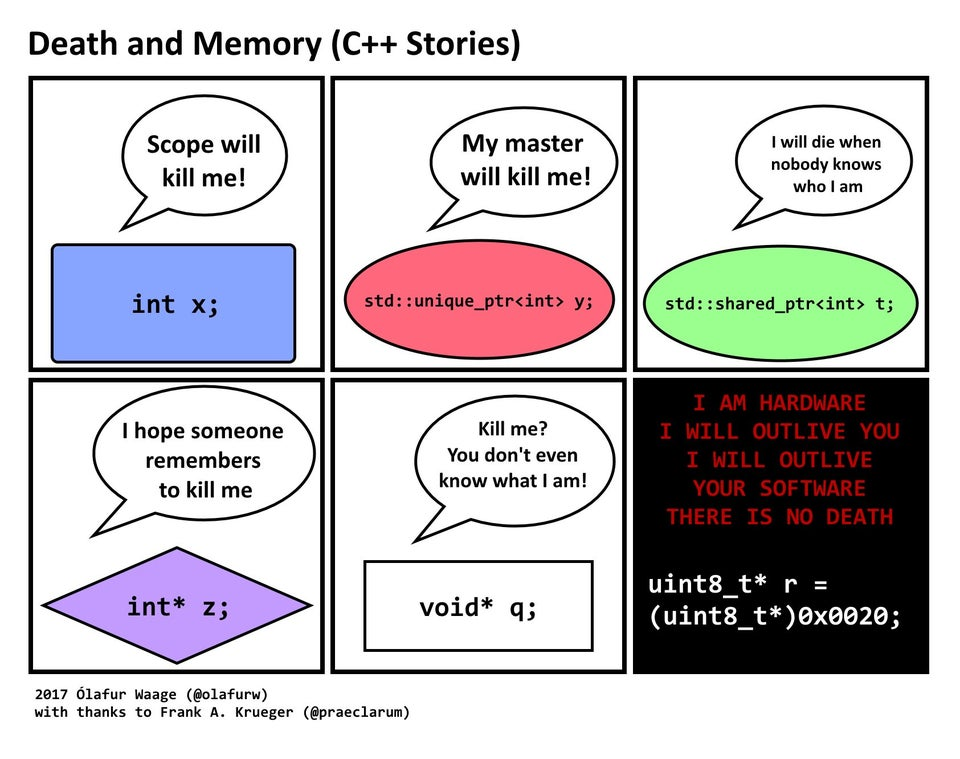
\includegraphics[width=1\textwidth, height=1\textheight, keepaspectratio]{./imgs/death_and_memory.jpg}
	\caption{La morte della memoria e RAII}
	\label{fig:death_and_memory}
\end{figure}

\subsection{Return Type Resolver}

\textsf{\small \textbf{Definizione: } Il \textbf{Return Type Resolver}, o anche conosciuto come \emph{Return type overloading} è un idioma il cui intento è quello di dedurre il tipo della variabile inizializzata o da assegnare.} \\

\textsf{\small Il problema: } \\

\begin{lstlisting}
	#include <iostream>
	#include <string>
	
	int fromString(const char *str) { return std::stoi(str); }
	float fromString(const char* str) { return std::stoi(str); } // Errore
\end{lstlisting}

\textsf{\small Una funzione non può essere \emph{overloaddata} solo dal suo tipo di ritorno.} \\

\begin{lstlisting}
	#include <iostream>
	#include <string>
	
	class fromString {
		const std::string str;
		public:
			fromString(const char* str) : str(str) {}
			template<typename type>
			operator type(){
				if constexpr(std::is_same_v<type, float>) return stof(str);
				else if(std::is_same_v<type, int>) return stoi(str);
			}
	};

	int main()
	{
		// Funzionerà con C++17 e oltre perché ha is\_same\_v
		int iStr = fromString("321");
		float fStr = fromString("654.987");
		return 0;
	}
\end{lstlisting}

%TODO: magari scrivere in basi del linguaggio o anche qui cos'è 'if constexpr'.

\begin{itemize}
	\item \textsf{\small Quando usi \textbf{nullptr} serve per dedurre il corretto tipo dipendendo dal puntatore a cui sta assegnando.}
	\item \textsf{\small Si può anche superare questa limitazione nel modo in cui abbiamo visto sopra.}
	\item \textsf{\small \textbf{Return Type Resolver} può anche essere usato per fornire un'interfaccia generale per l'assegnamento, indipendente dall'oggetto a cui è stato assegnato.}
\end{itemize}

\subsection{Type Erasure}

\textsf{\small \textbf{Definizione: } \textbf{Type Erasure}, o anche conosciuto come \emph{Duck-typing} serve per generare dei container che possono gestire una varietà di tipi.} \\

\textsf{\small Questo può essere implementato attraverso: \emph{void*}, \emph{templates}, \emph{polimorfismo}, \emph{union}, \emph{proxy class}, eccetera.} \break

\begin{itemize}
	\item \textsf{\small Il C++ è un linguaggio \emph{statically typed} con uno \emph{typing} forte. In questi tipi di linguaggi, la tipologia dell'oggetto è conosciuta a compile-time.} %TODO: magari spiegare meglio la parte del 'statically typed' con forte 'typing'
	\item \textsf{\small Quindi il tipo di un oggetto, dopo la compilazione, non cambia.}
	\item \textsf{\small Per ovviare a questo esistono vari containers come: \emph{std::any} (C++17), \emph{std::variant} (C++17), \emph{std::function} (C++11), eccetera.}
\end{itemize}

\textsf{\small Quindi esistono varie tecniche per implementare questo: } \\

\subsubsection{Type erasure usando void* (come nel C)}

\begin{lstlisting}
	void qsort(void* base, size_t num, size_t size, int(*comapare)(const void*, const void*));
\end{lstlisting}

\textsf{\small Lo svantaggio è che non è sicuro e separa la funzione `compare` necessaria per ogni tipo.} \\

\subsubsection{Type erasure usando i templates}

\begin{lstlisting}
	template <class RandomAccessIterator>
		void sort(RandomAccessIterator first, RandomAccessIterator last);
\end{lstlisting}

\textsf{\small Lo svantaggio: potrebbe portare all'istanzione di molte funzioni template e quindi di tempi di compilazione più lunghi. } \\

\subsubsection{Type erasure usando il polimorfismo}

\begin{lstlisting}
	class Base { 
		public:
			virtual void method() = 0; 
	};
	
	class C : Base { 
		public:
			void method() { cout << "classe C\n"; } 
	};

	class D : Base { 
		public:
			void method() { cout << "classe D\n"; } 
	};
	
	// Non vediamo un tipo concreto (viene cancellato) anche se lo si può castare con il dynamic\_cast.
	void call(Base* ptr) 
	{ 
		ptr->method(); 
	};
\end{lstlisting}

\textsf{\small Lo svantaggio è che costa a livello di runtime (dynamic dispatch, indirection, vtable, eccetera.)} \\

\subsubsection{Type erasure usando le union}

\begin{lstlisting}
	class Data {
		public:
			int x;
	};
	
	union U {
		Data d;         // occupa 1 byte
		std::int32_t n; // occupa 4 bytes
		char c;         // occupa 1 byte
		
		~U() {}         // ha bisogno di sapere il tipo correntemente attivo.
	}; // un'istanza di U occupa in totale 4 bytes.

	int main()
	{
		U u; // creo un'istanza chiamata u della union U.
		
		u.c = 's';
		u.d.x = 3;
		
		std::cout << "u.c: " << u.c << std::endl; //Output: u.c: s
		std::cout << "u.d.x: " << u.d.x << std::endl; //Output: u.d.x: 3
		return 0;
	}
\end{lstlisting}

\textsf{\small Lo svantaggio è che non è sicuro a livello di tipo (\emph{type-safe}).} \\

\subsubsection{Type erasure usando i containers generici}

\begin{lstlisting}
	#include <iostream>
	#include <memory>
	
	struct any 
	{
		struct base {};
		
		template<typename T>
		struct inner: base{
			inner(T t): m_t{std::move(t)} {}
			T m_t;
			static void type() {}
		};
		
		any(): m_ptr{nullptr}, typePtr{nullptr} {}
		
		template<typename T>
		any(T && t): m_ptr{std::make_unique<inner<T>>(t)}, typePtr{&inner<T>::type} {}
		
		template<typename T>
		any& operator=(T&& t){
			m_ptr = std::make_unique<inner<T>>(t); 
			typePtr = &inner<T>::type;
			return *this;
		}
		
		private:
		template<typename T>
		friend T& any_cast(const any& var);
		
		std::unique_ptr<base> m_ptr = nullptr;
		void (*typePtr)() = nullptr;
	};
	
	template<typename T>
	T& any_cast(const any& var)
	{
		if(var.typePtr == any::inner<T>::type)
		return static_cast<any::inner<T>*>(var.m_ptr.get())->m_t;
		throw std::logic_error{"Bad cast!"};
	}
	
	int main()
	{
		any var(10);
		std::cout << any_cast<int>(var) << std::endl;
		
		var = std::string{"some text"};
		std::cout << any_cast<std::string>(var) << std::endl;
		
		return 0;
	}
\end{lstlisting}

\textsf{\small Da notare come stiamo usando la funzione statica vuota \emph{inner<T>::type} per determinare l'istanza del template in \emph{any\_cast<T>}.} \\

\textsf{\small Questo è usato per gestire molteplici tipi di valori di ritorno dalle funzioni (Anche se non è raccomandato).} \\

\begin{figure}[H]
	\centering
	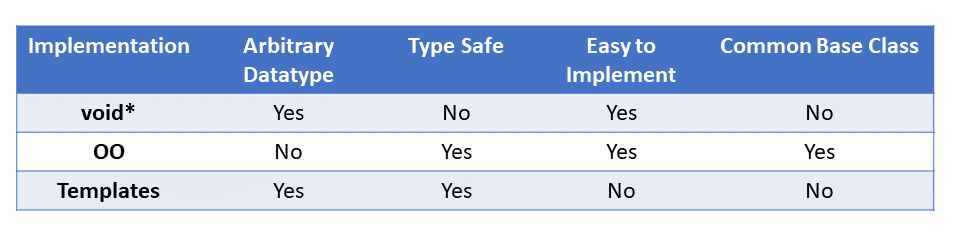
\includegraphics[width=1\textwidth, height=1\textheight, keepaspectratio]{./imgs/type_erasure.png}
	\caption{Type Erasure}
	\label{fig:type_erasure}
\end{figure}

\subsection{CRTP}

\textsf{\small \textbf{Definizione: } Il \textbf{CRTP} (\emph{\textbf{C}uriously \textbf{R}ecurring \textbf{T}emplate \textbf{P}attern}), o anche conosciuto come \emph{Upside-down inheritance} o \emph{Static polymorphism} è utilizzato per ottenere il polimorfismo statico.} \\

\textsf{\small Per ottenere questo fa uso della specializzazione delle classi template (\emph{base class template specialization}).} \break

\textsf{\small Problema: } \\

\begin{lstlisting}
	#include <iostream>
	
	struct obj_type_1
	{
		bool operator<(const value &rhs) const {return m_x < rhs.m_x;}
		// bool operator==(const value \&rhs) const;
		// bool operator!=(const value \&rhs) const;    
		// e la lista va avanti..
		private:
		// dati membri da comparare
	};
	
	struct obj_type_2
	{
		bool operator<(const value &rhs) const {return m_x < rhs.m_x;}
		// bool operator==(const value \&rhs) const;
		// bool operator!=(const value \&rhs) const;    
		// e la lista va avanti..
		private:
		// dati membri da comparare.
	};
	
	struct obj_type_3 { }
	struct obj_type_4 { }
	// e la lista va avanti..
\end{lstlisting}

\begin{itemize}
	\item \textsf{\small Per ogni oggetto comparabile, c'è bisogno di un rispettivo operatore di comparazione, il che è ridondante perché se abbiamo l'operatore <, possiamo \emph{overloaddare} gli altri operatori basandoci su quello.}
	\item \textsf{\small Quindi, l'operatore < è l'unico operatore che possiede l'informazione del tipo, altri operatori possono essere fatti indipendenti per questioni di riusabilità.}
	%\item \textsf{\small }
\end{itemize}

\textsf{\small La soluzione: } \\

\textsf{\small L'implementazione è semplice: \emph{separare le funzionalità dei tipi dipendenti e indipendenti e legare le funzionalità del tipo indipendente con la classe base usando la \emph{self-referencing template} (template a se stesso)}.} \\

\begin{lstlisting}
	#include <iostream>
	
	template <class derived>
	struct compare {};
	
	struct value : compare<value> {
		int m_x;
		value(int x) : m_x(x) {}
		bool operator<(const value &rhs) const { return m_x < rhs.m_x; }
	};
	
	template <class derived>
	bool operator > (const compare<derived> &lhs, const compare<derived> &rhs) {
		// static\_assert(std::is\_base\_of\_v<compare<derived>, derived>); // Compile time safety measures
		return (static_cast<const derived&>(rhs)<static_cast<const derived&>(lhs));
	}
	
	/*  Lo stesso vale per gli altri operatori
	== :: returns !(lhs < rhs) and !(rhs < lhs)
	!= :: returns !(lhs == rhs)
	>= :: returns (rhs < lhs) or (rhs == lhs)
	<= :: returns (lhs < rhs) or (rhs == lhs) 
	*/
	
	// Ora non c'è più bisogno di scrivere gli operatori di comparazione per ogni classe.
	// Scriviamo solo il tipo dipendente `operator <` \& usiamo il CRTP.
	int main() {   
		value v1{5}, v2{10};
		std::cout << std::boolalpha << "v1 > v2: " << (v1 > v2) << '\n'; //Output: v1 > v2: false
		return 0;
	}
\end{lstlisting}

\textsf{\small \textbf{CRTP} è ampiamente usata per il polimorfismo statico senza sostenere il costo del meccanismo di \emph{virtual dispatch}. Consideriamo il seguente codice, senza l'uso di \textbf{virtual} e continuando ad ottenere le funzionalità del polimorfismo statico.} \\

\begin{lstlisting}
	#include <iostream>
	
	template<typename specific_animal>
	class animal {
		public:
			void who() { implementation().who(); }
		private:
		specific_animal& implementation() {return *static_cast<specific_animal*>(this);}
	};
	
	class dog : public animal<dog> {
		public:
			void who() { std::cout << "dog" << std::endl; }
	};
	
	class cat : public animal<cat> {
		public:
			void who() { std::cout << "cat" << std::endl; }
	};
	
	template<typename specific_animal>
	void who_am_i(animal<specific_animal> & animal) {
		animal.who();
	}
	
	int main()
	{
		cat c;
		c.who(); //Output: cat
		return 0;
	}
\end{lstlisting}

\textsf{\small \textbf{CRTP} può anche essere usato per l'ottimizzazione e permette anche la riusabilità del codice.} \\

\textsf{\small Con C++20 risolviamo anche con lo \textbf{spaceship operator} <=> (default comparisons)/ \emph{three-way-comparison operator}.} \\

%TODO: magari approfondire lo spaceship operator aggiunto con C++20 (fare una subsubsection)

\subsubsection{3-way comparison operator | Spaceship Operator}

\textsf{\small Con il C++20 è stato aggiunto l'operatore \emph{three-way-comparator} \textbf{<=>} chiamato lo \textbf{spaceship operator}.} \\

\textsf{\small Questo operatore determina per due oggetti \emph{A} e \emph{B} se \emph{A < B}, \emph{A = B} o \emph{A > B}.} \\

\textsf{\small Inoltre, una funzione \emph{three-way-comparison} è una funzione che darà l'intera relazione in una query. Tradizionalmente, una funzione del genere è \emph{strcmp()}, date due stringhe restituisce un intero dove: } \\

\begin{itemize}
	\item \textsf{\small < 0 significa che la prima stringa è minore.}
	\item \textsf{\small == 0 significa che sono uguali.}
	\item \textsf{\small > 0 significa che la prima stringa è maggiore.}
\end{itemize}

\textsf{\small Può dare uno di questi tre risultati e quindi per questo è chiamata \emph{three-way-comparison}.} \\

\begin{tabular}{|c|c|}
	\hline
	\textbf{Equality} & \textbf{Ordering} \\
	\hline
	\textsf{\small \textbf{Primario}: ==} & \textsf{\small <=>} \\
	\hline
	\textsf{\small \textbf{Secondario}: !=} & \textsf{\small <, >, <=, >=} \\
	\hline
\end{tabular}

\begin{lstlisting}
	(A <=> B) < 0 // è vera se A < B.
	(A <=> B) > 0 // è vera se A > B.
	(A <=> B) == 0 // è vera se A e B sono uguali.
\end{lstlisting}

\textsf{\small Esempio: } \\

\begin{lstlisting}
	#include <iostream>
	
	int main()
	{
		float a = -0.0;
		float b = 0.0;
		
		auto compare = a <=> b;
		
		if(comapre < 0)
		{
			std::cout << "-0.0 è minore di 0.0" << std::endl;
		} else if(compare == 0){
			std::cout << "-0.0 e 0.0 sono uguali." << std::endl;
		} else {
			std::cout << "-0.0 è maggiore di 0.0" << std::endl;
		}
	
		//Output: -0.0 e 0.0 sono uguali.
		return 0;
	}
\end{lstlisting}

\subsection{Virtual Constructor}

\textsf{\small \textbf{Definizione: } Il \textbf{Costruttore Virtuale}, o anche conosciuto come \emph{Factory method/design-pattern}, ha lo scopo di creare una copia o un nuovo oggetto senza sapere di concreto il suo tipo.} \\

\textsf{\small Per fare questo sfruttiamo le funzioni \emph{overloaded} con l'assegnamento polimorfico.} \break

\textsf{\small Il problema: } \\

\begin{itemize}
	\item \textsf{\small C++ supporta la distruzione di oggetti polimorfici usando il \textbf{distruttore virtuale} della classe base, ma l'equivalente supporto per la creazione e la copiatura di oggetti manca visto che non supporta i \textbf{costruttori virtuali}, ma ci sono i \textbf{copy constructors}.}
	\item \textsf{\small Inoltre, non puoi creare un oggetto a meno che sai il suo tipo, perché il compilatore deve sapere l'ammontare di spazio da allocare. Per lo stesso motivo, la copiatura di un oggetto richiede anch'esso di sapere il suo tipo a compile-time.}
\end{itemize}

\begin{lstlisting}
	#include <iostream>
	
	class Animal {
		public:
			virtual ~Animal(){ std::cout<<"~animal\n"; }
	};
	
	class Dog : public Animal {
		public:
			~Dog(){ std::cout<<"~dog\n"; }
	};
	
	class Cat : public Animal {
		public:
			~Cat(){ std::cout<<"~cat\n"; }
	};
	
	void who_am_i(Animal *who) {
		
		// Come `creare` l'oggetto dello stesso tipo, ovvero puntato da who ?
		// Come `copiare` l'oggetto dello stesso tipo, ovvero puntato da who ?
		
		delete who; // si può cancellare gli oggetti puntati da who.
	}
\end{lstlisting}

\textsf{\small La soluzione: } \\

\begin{itemize}
	\item \textsf{\small La tecnica del \textbf{Costruttore Virtuale} permette la creazione polimorfica e la copiatura di oggetti delegando la creazione e la copiatura dell'oggetto alla classe derivata attraverso l'uso di funzioni virtuali.}
	\item \textsf{\small Il seguente codice non solo implementa il \textbf{costruttore virtuale}, ma anche il \textbf{virtual copy constructor}.}
\end{itemize}

\begin{lstlisting}
	#include <iostream>
	#include <memory>
	
	class Animal {
		public:
			virtual ~Animal() = default;
			virtual std::unique_ptr<Animal> create() = 0;
			virtual std::unique_ptr<Animal> clone() = 0;
	};
	
	class Dog : public Animal {
		public:
			std::unique_ptr<Animal> create() { return std::make_unique<Dog>(); }
			std::unique_ptr<Animal> clone() { return std::make_unique<Dog>(*this); }
	};
	
	class Cat : public Animal {
		public:
			std::unique_ptr<animal> create() { return std::make_unique<Cat>(); }
			std::unique_ptr<animal> clone() { return std::make_unique<Cat>(*this); }
	};
	
	void who_am_i(Animal *who) {
		auto new_who = who->create(); // `create` l'oggetto dello stesso tipo, ovvero puntato da who ?
		
		auto duplicate_who = who->clone(); // `copy` l'oggetto dello stesso tipo, ovvero puntato da who ?    
		
		delete who; //si può cancellare l'oggetto puntatore da who.
	}
\end{lstlisting}

\textsf{\small Fornisce un'interfaccia generica per produrre/copiare una varietà di classi usando solo una classe.} \\

\subsection{SFINAE}

\label{SFINAE}

\textsf{\small \textbf{Definizione: } \textbf{SFINAE} (\emph{\textbf{S}ubstitution \textbf{F}ailure \textbf{I}s \textbf{N}ot \textbf{A}n \textbf{E}rror}) ha lo scopo di filtrare le funzioni che non producono delle istanze template valide da un insieme di funzioni \emph{overloaded}.} \\

\textsf{\small Otteniamo questo in maniera automatica dal compilatore oppure sfruttando \textbf{std::enable\_if}.} \break

\textsf{\small Motivazioni: } \\

\begin{itemize}
	\item \textsf{\small È una feature del linguaggio (non un idioma).}
	\item \textsf{\small Durante l'\emph{overload} delle funzioni template, quando la sostituzione del tipo specificato o dedotto dei parametri del template falliscono, la specializzazione viene scartata invece che causare un errore di compilazione.}
	\item \textsf{\small Il fallimento della sostituzione (\emph{Substitution Failure}) accade quando il tipo o l'espressione sono mal formati.}
\end{itemize}

\begin{lstlisting}
	#include <iostream>
	
	template<class T>
	void func(T* t){ // Single overload set
		if constexpr(std::is_class_v<T>){ std::cout << "T è un tipo definito dall'utente\n"; }
		else { std::cout << "T è un tipo primitivo\n"; }
	}
	
	int primitive_t = 6;
	struct {char var = '4';}class_t;
	
	int main()
	{
		func(&class_t);
		func(&primitive_t);
		
		//Output: T è un tipo definito dall'utente
		//Output: T è un tipo primitivo
		return 0;
	}
\end{lstlisting}

\textsf{\small Immagina di voler creare due insiemi (basati sui tipi primitivi e sui tipi definiti dall'utente separatamente) di una funzione che ha la stessa \emph{signature}? (tipo di ritorno, nome, parametri della funzione).} \\

\textsf{\small Soluzione: } \\

\begin{lstlisting}
	#include <iostream>
	
	template<class T, typename = std::enable_if_t<std::is_class_v<T>>>
	void func(T* t){
		std::cout << "T è un tipo definito dall'utente.\n";
	}
	
	template<class T, std::enable_if_t<std::is_integral_v<T>, T> = 0>
	void func(T* t){ // la signature della funzione non è modificata.
		std::cout << "T è un tipo primitivo.\n";
	}
\end{lstlisting}

\textsf{\small Il code snippet (frammento di codice) sopra è un esempio di come sfruttare \textbf{SFINAE} attraverso l'uso di \textbf{std::enable\_if}, nella quale le istanze template diventeranno uguali a \emph{void func<(anonymous), void>((anonymous) * t)} e \emph{void func(int *t)}} \break

\textsf{\small Assieme con \textbf{std::enable\_if}, \textbf{SFINAE} è ampiamente usata nel \emph{template metaprogramming}.} \\

\textsf{\small La libreria standard ha anche influenzato \textbf{SFINAE} nel \emph{utilities} \textbf{<type\_traits>}.} \\

\begin{lstlisting}
	#include <iostream>
	
	template<typename T>
	class is_class_type {
		template<typename C> static char test(int C::*);    
		template<typename C> static double test(...);
		public:
		enum { value = sizeof(is_class_type<T>::test<T>(0)) == sizeof(char) };
	};
	
	struct class_t{};
	
	int main()
	{
		std::cout<<is_class_type<class_t>::value<< std::endl; //Output: 1
		std::cout<<is_class_type<int>::value<< std::endl; //Output: 0
		return 0;
	}
\end{lstlisting}

\textsf{\small Senza \textbf{SFINAE} avresti un errore dal compilatore, qualcosa del tipo: <<\emph{0 cannot be converted to member pointer for a non-class type int}>> visto che l'\emph{overload} di test differisce solo del tipo di ritorno e visto che int non è una classe non può avere membro puntatore di tipo \emph{int int::*}.} \\

\newpage %TODO: questo \newpage per via degli spazi bianchi sopra.

\begin{figure}[H]
	\centering
	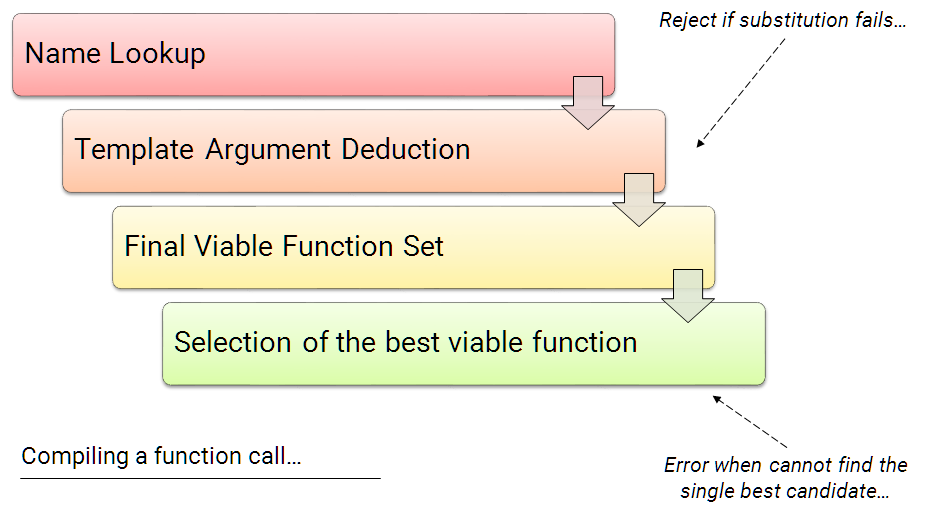
\includegraphics[width=1\textwidth, height=1\textheight, keepaspectratio]{./imgs/SFINAE.png}
	\caption{SFINAE}
	\label{fig:SFINAE}
\end{figure}

\textsf{\small \textbf{SFINAE} è stato praticamente rimpiazzato dai \textbf{Concepts} del \textbf{C++20} che fanno la stessa cosa, ma molto meglio. Guardare pag.\textbf{\pageref{concepts}} del capitolo \emph{Le gemme degli Algoritmi}.} \\ %TODO: dovrei forse metterlo all'inizio della subsection?

\subsection{Proxy}

\textsf{\small \textbf{Definizione: } Il \textbf{Proxy}, o anche conosciuto come \emph{operator[] (subscript) proxy}, \emph{double/twice operator overloading} è un \emph{design pattern} il cui intento è quello di ottenere funzionalità pratiche attraverso una classe \emph{middleware}.} \\

\textsf{\small Quindi, il \textbf{Proxy} è una classe che fornisce un'interfaccia modificata ad un'altra classe ed è usata per implementare il \textbf{Proxy Patern}: nel quale un oggetto è un intermediario per qualche altro oggetto.} \\

\textsf{\small Implementiamo questo attraverso una classe \emph{temporanea/proxy}.} \break

\begin{itemize}
	\item \textsf{\small È per via del \emph{subscript operator} (operator[]), ma è possibile che anche il tipo/classe che si frappone nello scambio di dati sia proxy. }
	\item \textsf{\small Abbiamo già visto un esempio di questo nel \textbf{type-erasure} (classe any::inner<>).}
	\item \textsf{\small Vedremo un ulteriore esempio ora con l'\textbf{operator[]}}
\end{itemize}

\begin{lstlisting}
	#include <iostream>
	
	template <typename T = int>
	struct arr2D{
		private:
		struct proxy_class{
			proxy_class(T *arr) : m_arr_ptr(arr) {}
			// operator[]
			T &operator[](uint32_t idx) { return m_arr_ptr[idx]; }
			
			private:
			T *m_arr_ptr;
		};
		
		T m_arr[10][10];
		
		public:
		arr2D::proxy_class operator[](uint32_t idx) { return arr2D::proxy_class(m_arr[idx]); }
	};
	
	int main()
	{
		arr2D<> arr;
		arr[0][0] = 1;
		std::cout << arr[0][0]; //Output: 1
		return 0;
	}
\end{lstlisting}

\textsf{\small Per creare delle funzionalità pratiche come \emph{double operator overloading}, \emph{std::any}, eccetera.} \\

\newpage %TODO: questo \newpage per gli spazi bianchi.

\begin{figure}[H]
	\centering
	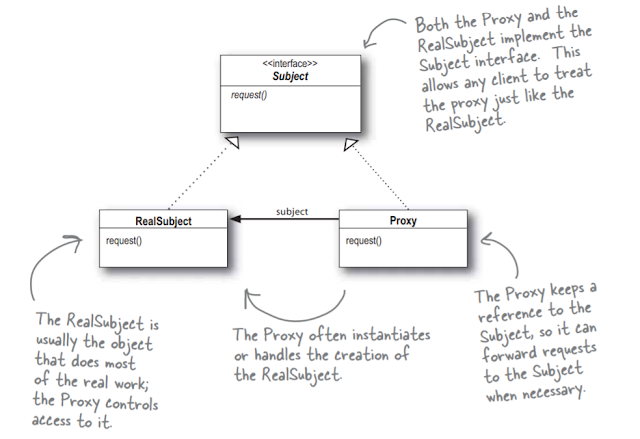
\includegraphics[width=1\textwidth, height=1\textheight, keepaspectratio]{./imgs/Design_Patterns/Proxy_Pattern.png}
	\caption{Proxy Pattern}
	\label{fig:Proxy_Pattern}
\end{figure}

% ------------------------------ FINE CAPITOLO ---------------------------------------